%!TEX root = thesis.tex

\chapter{Baseline system} %TODO
\label{ch:Content1}


A system for symbol recognition was already written and is described in \cite{Kirsch}.
It uses an algorithm called greedy matching which is similar to \Gls{DTW}.

The Greedy Matching algorithm takes two series of points $(A, B)$ and matches
the first points $(a,b)$ of $A$ to $B$. The distance that point had to be moved is
measured. Afterwards, it tries to match the next point $a'$ of $A$ to $b$ as
well as the next point $b'$ of $B$ and $b'$ to $a$. It takes the matching in
which the points had to be moved the shortest distance and continues like that.

Pseudocode is on \cpageref{alg:greedy-matching}.

%!TEX root = thesis.tex
\chapter{Data, Preprocessing and Features}\label{ch:preprocessing}

\begin{wrapfigure}{r}{7cm}
  \vspace{-35pt}
  \begin{center}
    \newcommand*{\xMin}{0}%
\newcommand*{\xMax}{6}%
\newcommand*{\yMin}{0}%
\newcommand*{\yMax}{6}%
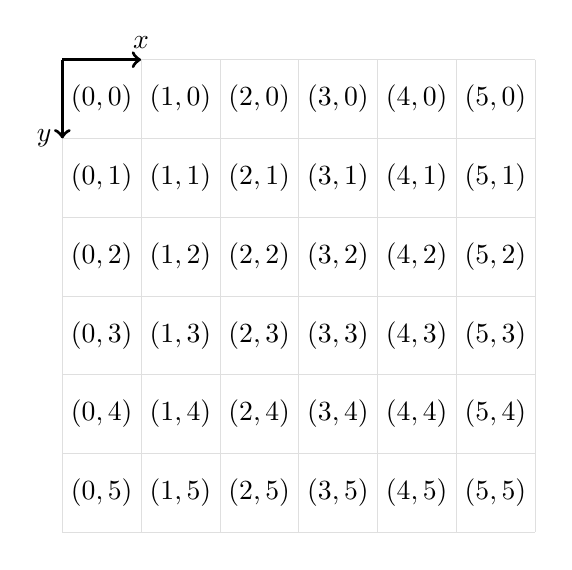
\begin{tikzpicture}[y=-1cm]
    \foreach \i in {\xMin,...,\xMax} {
        \draw [very thin,gray!25] (\i,\yMin) -- (\i,\yMax)  node [below] at (\i,\yMin) {};
    }
    \foreach \i in {\yMin,...,\yMax} {
        \draw [very thin,gray!25] (\xMin,\i) -- (\xMax,\i) node [left] at (\xMin,\i) {};
    }
    \draw[->, very thick] (0,0) -- (1,0) node[above] {$x$};
    \draw[->, very thick] (0,0) -- (0,1) node[left] {$y$};
    \foreach \x in {\xMin,...,5} {
        \foreach \y in {\yMin,...,5} {
            \node at ({\x+0.5},{\y+0.5}) {$(\x, \y)$};
        }
    }
\end{tikzpicture}
  \end{center}
  \vspace{-20pt}
  \caption{HTML5 canvas plane. Each step is one pixel. There cannot be non-integer
           coordinates.}
  \label{fig:canvas-plane}
  \vspace{-10pt}
\end{wrapfigure}

The data that was used for all experiments was collected with
\href{http://write-math.com}{write-math.com}, a website designed solely for
this purpose. This website makes use of HTML5 canvas elements. Those elements
can be used to track fingers or a mouse coursor touching the canvas, moving
and lifting. The origin is at the upper left corner and get bigger to the right
($x$-coordinate) and to the bottom ($y$-coordinate).

The data is stored and shared in JSON format. Each handdrawing is stored as a
list of lines, where each line consists of tuples $(x(t), y(t), t)$, where $x$
and $y$ are canvas coordinates and $t$ is a timestamp in seconds. This timestamp
gives the time in milliseconds from 1970.

The time resolution between points as well as the resolution of the image
depends on the device that was used. However, most symbols have a time
resolution of about $\SI{20}{\milli\second}$ and are within a bounding box of a
$250 \text{px} \times 250 \text{px}$ square.

\section{Preprocessing}\label{sec:preprocessing}
\subsection{Normalization: Scaling, shifting and resampling}
In \cite{Kirsch} the datapoints were scaled to fit into a unit square while
keeping their aspect ratio. Afterwards, the points were shifted to
the $(0, 1) \times (0, 1)$ unit square. The algorithm is given in pseudocode on
\cpageref{alg:scale-and-shift}. It was shown in \cite{Kirsch,Huang09} that
this kind of preprocessing boosts classification accuracy significantly.

Another method to normalize data is resampling, sometimes also called
stroke length normalization.
\cite{Guyon91} resampled characters and digits to 81 points each, where different
lines were also connected by \enquote{pen-up} segments. They resampled to get
points regulary spaced in arc length, not in time. \cite{ICASSP-94} also
resampled data to get points regulary spaced in arc length, but they encoded
speed as an extra feature.

\subsection{Noise reduction}
The following list of noise reduction methods was created by \cite{Tappert90}
and is still up-to-date.\nopagebreak
\begin{itemize}
    \item \textbf{Smoothing} can be done in multiple ways. An approach that was
          used quite often is applying a weighted average
          \cite{Groner66,Division87,Arakaw83}. \cref{alg:weighted-average-smoothing}
          describes in pseudocode how to implement weighted average smoothing.
    \item \textbf{Wild-point detection} and deletion or replacement of 
          wild points with the average of neighboring points\cite{Division87},
    \item \textbf{Filtering} is the process of removing points by some criteria.
          Those criteria include:
          \begin{itemize}
              \item Duplicate points,
              \item Enforcing a minimal distance between consecutive 
                    points\cite{Tappert90}.
              \item Enforcing a minimal change in direction\cite{Tappert90}.
          \end{itemize}
          An idea that seemingly nobody has tried before is applying the
          Douglas-Peucker algorithm for filtering dots.
    \item \textbf{Dehooking} [TODO: Image of hook]
    \item \textbf{Dot reduction} reduces dots to single points. Sometimes
          multiple points get recorded although the user wanted to make only
          a single point, e.g. for one of the following symbols:
          $\cdot$, ., $\dots$, $\vdots$, $\ddots$, i, ä, ö, ü.
          This can be detected by calculating
          the maximum distance $d$ two points in a stroke have. If $d$ is
          smaller than a threshold $\theta$, then it is a single point.
          In that case all points of the line get reduced to a single dot.
          This dot could be the center of mass of all points in the stroke.
    \item \textbf{Stroke connection} might be used if the distance between
          pen-up and pen-down is below a threshold.
    \item \textbf{Deskewing} corrects character slant.
    \item \textbf{Baseline drift correction} moves words to be on a baseline.
\end{itemize}

Wild points are points that appear within a sequence of points of a stroke. They
that were not caused by the pen, but by a hardware error. They are characterized
by a very high velocity and sharp angles.

\section{Features}\label{sec:features}
A number of different features have been suggested so far for on-line handwriting
recognition. They can be grouped into local features and global features.
Local features apply to a given point on the drawing plane and sometimes even
only to point on the drawn curve whereas global features apply to a complete
line or even the complete image.

\subsection{Local features}
\begin{itemize}
    \item Coordinates of the current point\cite{Guyon91}
    \item Speed\cite{Huang09,ICASSP-94}
    \item Binary pen pressure\cite{Kosmala98,Kosmala11,ICASSP-94}
    \item Direction\cite{Manke95,Huang06}
    \item Curvature\cite{Groner66,Manke95,ICASSP-94,Guyon91}
    \item Bitmap-environment\cite{Manke95}
    \item Hat-Feature\cite{ICASSP-94,Manke00}
\end{itemize}

\cite{Kosmala98,Kosmala11} suggest that speed is a bad feature, because it \enquote{highly inconsistent}.

The \textbf{direction} $\text{dir}$ at the point $i$ can be described by the vector 
$(\cos \theta(i), \sin \theta(i))$ as described in \cite{Guyon91}.

\begin{align}
    \cos \theta(i) &= \frac{\Delta x^{(i)}}{\Delta s^{(i)}}\\
    \sin \theta(i) &= \frac{\Delta y^{(i)}}{\Delta s^{(i)}}
\end{align}

where

\begin{align}
    \Delta x (i) &= x^{(i+1)} - x^{(i-1)}\\
    \Delta y (i) &= y^{(i+1)} - x^{(i-1)}\\
    \Delta s (i) &= \sqrt{\Delta (x^{(i)})^2 + \Delta y (y^{(i)})^2}
\end{align}

The \textbf{curvature} $\phi$ of the point $i$ can be described by the
angle of the two neighboring points:

% TODO!
% \begin{align}
%     \text{cur}(i) &= \text{dir}(i-1)
% \end{align}

\subsection{Global features}
\begin{itemize}
    \item Re-curvature\cite{Huang06} (TODO: Explain (all))
    \item Center point\cite{Huang06}
    \item Stroke length\cite{Huang06}
    \item Number of strokes\cite{Huang09}
    \item Pseudo-Zernike Features (TODO: Really global? What is it?)\cite{Khotanzad}
    \item Shadow Code Features\cite{Khotanzad}
\end{itemize}
%!TEX root = thesis.tex
\chapter{Artificial Neural Nets}\label{ch:ANNs}

\Glspl{ANN} are models for classification that were inspired by the brain.
They consist of artificial neurons and have a lot of different subtypes like
Feed Forward Neural Nets.

%!TEX root = thesis.tex
\section{Artificial neurons}\label{sec:artificial-neurons}
%% ===========================

Artificial neurons are inspired by biological neurons. Signals are send within 
the cell by charged particles, so called \textit{ions}. But before a biological
neuron sends a signal, a threshold charge has to be reached at the axon
hillock. This threshold charge is called \textit{action potential}. The action
potential can be reached by multiple factors, but the one I want to focus on
are charges send by other neurons. Depending on where the other axon terminals
are located and how long the distance to the axon hillock is, the signal contributes
more or less to reaching the action potential. After that, it simply sends a
signal.

\begin{figure}[ht]
    \centering
    \subfloat[Biological Neuron]{
        \includegraphics*[width=0.48\linewidth, keepaspectratio]{figures/biological-neuron.jpg} 
        \label{fig:biological-neuron}
    }%
    \subfloat[Artificial Neuron]{
        \resizebox{0.45\linewidth}{!}{
\tikzstyle{inputNode}=[draw,circle,minimum size=10pt,inner sep=0pt]
\tikzstyle{stateTransition}=[->, thick]
\begin{tikzpicture}
    \node[draw,circle,minimum size=25pt,inner sep=0pt] (x) at (0,0) {$\Sigma$ $\varphi$};

    \node[inputNode] (x0) at (-2, 1.5) {$\tiny x_0$};
    \node[inputNode] (x1) at (-2, 0.75) {$\tiny x_1$};
    \node[inputNode] (x2) at (-2, 0) {$\tiny x_2$};
    \node[inputNode] (x3) at (-2, -0.75) {$\tiny x_3$};
    \node[inputNode] (xn) at (-2, -1.75) {$\tiny x_n$};

    \draw[stateTransition] (x0) to[out=0,in=120] node [midway, sloped, above=-2] {$w_0$} (x);
    \draw[stateTransition] (x1) to[out=0,in=150] node [midway, sloped, above=-2] {$w_1$} (x);
    \draw[stateTransition] (x2) to[out=0,in=180] node [midway, sloped, above=-2] {$w_2$} (x);
    \draw[stateTransition] (x3) to[out=0,in=210] node [midway, sloped, above=-2] {$w_3$} (x);
    \draw[stateTransition] (xn) to[out=0,in=240] node [midway, sloped, above=-2] {$w_n$} (x);
    \draw[stateTransition] (x) -- (1.5,0) node[right] {$o$};
    \draw[dashed] (0,-0.43) -- (0,0.43);
    \node (dots) at (-2, -1.15) {$\vdots$};
\end{tikzpicture}}
        \label{fig:artificial-neuron}
    }%
    \label{fig:artificial-and-biological-neuron}
    \caption{Both neurons receive weighted input, apply a function to that and give output}
\end{figure}

Artificial neurons are similar. They receive at least one input and give at
least one output. Those inputs might get weighted as well as the output.

The neurons apply a function to the sum of all weighted inputs. This function
is also called \textit{activation function}.

An artificial neuron using the unit step function (see \cref{f:unitstep}) is called
a \textit{perceptron}.


The artificial neuron sums all weighted inputs $x_i \cdot w_i$ up
             and applies its activation function $f$ to it.
%!TEX root = thesis.tex
\section{Multilayer Perceptron}\label{ch:Content2:sec:Section2}

\Glspl{MLP} are neural nets whichs neurons are structured in layers.
Each layer is fully connected with the next layer, but there are no other
connections between neurons.

\begin{figure}[ht]
    \centering
    %!TEX root = thesis.tex
\section{Multilayer Perceptron}\label{ch:Content2:sec:Section2}

\Glspl{MLP} are neural nets whichs neurons are structured in layers.
Each layer is fully connected with the next layer, but there are no other
connections between neurons.

\begin{figure}[ht]
    \centering
    \input{figures/feedforward.tex}
    \caption{Feedforward artificial neural network}
    \label{fig:feedforward}
\end{figure}

The red neurons in \cref{fig:feedforward} are input neurons, the green ones are
hidden neurons and the blue one is an output node. The gray neurons are bias neurons.
Bias neurons have a fixed output of $1$.

Usually, you have as many output neurons as you have classes. So in the case of
symbol recognition that would be about $\si{1076}$ neurons.

The number of input neurons is equal to the number of features.

Two neighboring layers of neurons are fully connected and have weights between
two layers. This means you can store those weights in form of matrices.
Assuming you have $n$ neurons in layer $i$ and $m$ neurons in layer $i + 1$,
you would have a matrix

\[W_{i} = \begin{pmatrix}
    w_{1,1} & w_{1,2} & \dots & w_{1,m}\\
    w_{2,1} & w_{2,2} & \dots & w_{2,m}\\
    w_{3,1} & w_{3,2} & \dots & w_{3,m}\\
    \vdots  &         & \ddots& \vdots \\
    w_{n,1} & w_{n,2} & \dots & w_{n,m}
\end{pmatrix}\]

This means you can easily get the input for layer $i+1$. As the input neurons
output is $x \in \mdr^{1 \times n}$ you can simply multiply $x \cdot W_1$
to get the output $x \cdot W_1 := \net_j \in \mdr^{1 \times m}$.

After that, you can apply the activation function $\varphi$ to $_i$.
As I assume that the activation function will be the same foreach node in the
same layer $l$, I will simply write $\varphi_l(o)$. This means that $\varphi_l$ is applied
componentwise to each $o_i$ with $i \in 1, \dots, m$.

So the output vector $o$ of a 3-layer (input, hidden, output) neural net can be
computed by

\[o = \varphi_2(\varphi_1(x \cdot W_{1,2}) \cdot W_{2,3})\]

The output of a general \gls{MLP} can be computed by

\begin{align*}
    \Phi(x, 1) &:= \varphi_{1}(x \cdot W_{1,2})\\
    \Phi(x, n) &:= \varphi_{n-1} \big (\Phi(x, n-1) \cdot W_{n-1, n} \big)
\end{align*}

\subsection{Supervised Training with Backpropagation}
The backpropagation algorithm is a supervised algorithm for training an
\gls{MLP}. This means the trainigset $T$ consists of tuples $(x, t)$
where $x$ is input and $t_x$ is the desired output.

The backpropagation algorithm first makes a forward pass to get to know what
the current output $o_x$ would be for each $(x, t_x) \in T$.
To evaluate how good the current \gls{MLP} is, an error function can be defined:

\begin{align*}
    E: \mdr^{n_1 \times n_2} \times \mdr^{n_2 \times n_3} \times \dots \times \mdr^{n_{m-1, m}} \rightarrow \mdr_{\geq 0}\\
    E_T(W) = \frac{1}{2} \sum_{(x, t_x) \in T} \sum_{k \in out} \left (t_{x}^{(k)} - o_{x}^{(k)} \right )^2
\end{align*}

where $n_i$ is the numer of neurons in the $i$-th layer and $m$ is the number
of layers and $out$ is the set of all output neurons.

This function is isomorphic to 

\[E: \mdr^{\sum_{i=2}^m n_{i-1} \cdot n_{i}} \rightarrow \mdr_{\geq 0}\]

This error should be minimized. As the error is the sum of non-negative values,
we will get a lower error by minimizing the error for a single training example.
However, note that those minimizations are not independant. This means, we could
get trapped in a local minimum.

The idea is to \enquote{go} into the direction in which the error $E$ decreases
most. This is the gradient and the process is thus called \textit{gradient descent}.

At this point we need to decide how far we want to go. If we make too big steps
in the direction of the gradient, we might overshoot. If we make too small steps,
the algorithm will take too long to get to the minimum. As reducing the error
is basically learning the number is called learning rate $\eta \in \mdr_{> 0}$.

So the algorithm is

\begin{algorithm}[h]
    \begin{algorithmic}
        \Function{backpropagate}{$T$, $W$}
            \While{True}
                \ForAll{$(x, t_x) \in T$}
                    \ForAll{node $i$}
                        \ForAll{nodes $j$ following $i$}
                            \State $\displaystyle w_{ij} \gets w_{ij} - \eta \frac{\partial E_{\Set{x}}}{\partial w_{ij}} (W)$
                        \EndFor
                    \EndFor
                \EndFor
            \EndWhile
        \EndFunction
    \end{algorithmic}
\caption{Backpropagate}
\label{alg:backpropagate}
\end{algorithm}

Computing the partial derivatives $\frac{\partial E_{\Set{x}}}{\partial w_{ij}}$
is not a trivial task. To do that, we have to take a closer look at the
error function:

Let $n$ be the number of layers of the \gls{MLP}.

\begin{align}
    \frac{\partial E_{\Set{x}}}{\partial w_{ij}}
    &= \frac{\partial}{\partial w_{ij}} \frac{1}{2} \sum_{(x, t_x) \in T} \sum_{k \in out} \left (t_{x}^{(k)} - o_{x}^{(k)} \right )^2\\
    &= \frac{1}{2} \sum_{(x, t_x) \in T} \sum_{k \in out} \frac{\partial}{\partial w_{ij}} \left (t_{x}^{(k)} - o_{x}^{(k)} \right )^2\\
    &= \frac{1}{2} \sum_{(x, t_x) \in T} \sum_{k \in out} 2 \left (t_{x}^{(k)} - o_{x}^{(k)} \right ) \cdot \frac{\partial}{\partial w_{ij}} \left (t_{x}^{(k)} - o_{x}^{(k)} \right )\\
    &= - \sum_{(x, t_x) \in T} \sum_{k \in out} \left (t_{x}^{(k)} - o_{x}^{(k)} \right ) \cdot \frac{\partial}{\partial w_{ij}} \left (\varphi_{n-1}(\Phi(x, n-1) \cdot W_{n-1,n})^{(k)} \right)
\end{align}

At this point, it doesn't get simpler except if you know where $w_{ij}$ is.
If $w_{ij}$ is for example a weight for an output node, you can apply the chain
rule\footnote{$(f(g))' = f'(g) \cdot g'$} once:

\begin{align}
    \frac{\partial E_{\Set{x}}}{\partial w_{ij}} &= - \sum_{(x, t_x) \in T} \sum_{k \in out} \left (t_{x}^{(k)} - o_{x}^{(k)} \right ) \cdot \left ( \frac{\partial}{\partial w_{ij}} \varphi_{n-1} \right )(\Phi(x, n-1) \cdot W_{n-1,n})^{(k)}\\
\end{align}
    \caption{Feedforward artificial neural network}
    \label{fig:feedforward}
\end{figure}

The red neurons in \cref{fig:feedforward} are input neurons, the green ones are
hidden neurons and the blue one is an output node. The gray neurons are bias neurons.
Bias neurons have a fixed output of $1$.

Usually, you have as many output neurons as you have classes. So in the case of
symbol recognition that would be about $\si{1076}$ neurons.

The number of input neurons is equal to the number of features.

Two neighboring layers of neurons are fully connected and have weights between
two layers. This means you can store those weights in form of matrices.
Assuming you have $n$ neurons in layer $i$ and $m$ neurons in layer $i + 1$,
you would have a matrix

\[W_{i} = \begin{pmatrix}
    w_{1,1} & w_{1,2} & \dots & w_{1,m}\\
    w_{2,1} & w_{2,2} & \dots & w_{2,m}\\
    w_{3,1} & w_{3,2} & \dots & w_{3,m}\\
    \vdots  &         & \ddots& \vdots \\
    w_{n,1} & w_{n,2} & \dots & w_{n,m}
\end{pmatrix}\]

This means you can easily get the input for layer $i+1$. As the input neurons
output is $x \in \mdr^{1 \times n}$ you can simply multiply $x \cdot W_1$
to get the output $x \cdot W_1 := \net_j \in \mdr^{1 \times m}$.

After that, you can apply the activation function $\varphi$ to $_i$.
As I assume that the activation function will be the same foreach node in the
same layer $l$, I will simply write $\varphi_l(o)$. This means that $\varphi_l$ is applied
componentwise to each $o_i$ with $i \in 1, \dots, m$.

So the output vector $o$ of a 3-layer (input, hidden, output) neural net can be
computed by

\[o = \varphi_2(\varphi_1(x \cdot W_{1,2}) \cdot W_{2,3})\]

The output of a general \gls{MLP} can be computed by

\begin{align*}
    \Phi(x, 1) &:= \varphi_{1}(x \cdot W_{1,2})\\
    \Phi(x, n) &:= \varphi_{n-1} \big (\Phi(x, n-1) \cdot W_{n-1, n} \big)
\end{align*}

\subsection{Supervised Training with Backpropagation}
The backpropagation algorithm is a supervised algorithm for training an
\gls{MLP}. This means the trainigset $T$ consists of tuples $(x, t)$
where $x$ is input and $t_x$ is the desired output.

The backpropagation algorithm first makes a forward pass to get to know what
the current output $o_x$ would be for each $(x, t_x) \in T$.
To evaluate how good the current \gls{MLP} is, an error function can be defined:

\begin{align*}
    E: \mdr^{n_1 \times n_2} \times \mdr^{n_2 \times n_3} \times \dots \times \mdr^{n_{m-1, m}} \rightarrow \mdr_{\geq 0}\\
    E_T(W) = \frac{1}{2} \sum_{(x, t_x) \in T} \sum_{k \in out} \left (t_{x}^{(k)} - o_{x}^{(k)} \right )^2
\end{align*}

where $n_i$ is the numer of neurons in the $i$-th layer and $m$ is the number
of layers and $out$ is the set of all output neurons.

This function is isomorphic to 

\[E: \mdr^{\sum_{i=2}^m n_{i-1} \cdot n_{i}} \rightarrow \mdr_{\geq 0}\]

This error should be minimized. As the error is the sum of non-negative values,
we will get a lower error by minimizing the error for a single training example.
However, note that those minimizations are not independant. This means, we could
get trapped in a local minimum.

The idea is to \enquote{go} into the direction in which the error $E$ decreases
most. This is the gradient and the process is thus called \textit{gradient descent}.

At this point we need to decide how far we want to go. If we make too big steps
in the direction of the gradient, we might overshoot. If we make too small steps,
the algorithm will take too long to get to the minimum. As reducing the error
is basically learning the number is called learning rate $\eta \in \mdr_{> 0}$.

So the algorithm is

\begin{algorithm}[h]
    \begin{algorithmic}
        \Function{backpropagate}{$T$, $W$}
            \While{True}
                \ForAll{$(x, t_x) \in T$}
                    \ForAll{node $i$}
                        \ForAll{nodes $j$ following $i$}
                            \State $\displaystyle w_{ij} \gets w_{ij} - \eta \frac{\partial E_{\Set{x}}}{\partial w_{ij}} (W)$
                        \EndFor
                    \EndFor
                \EndFor
            \EndWhile
        \EndFunction
    \end{algorithmic}
\caption{Backpropagate}
\label{alg:backpropagate}
\end{algorithm}

Computing the partial derivatives $\frac{\partial E_{\Set{x}}}{\partial w_{ij}}$
is not a trivial task. To do that, we have to take a closer look at the
error function:

Let $n$ be the number of layers of the \gls{MLP}.

\begin{align}
    \frac{\partial E_{\Set{x}}}{\partial w_{ij}}
    &= \frac{\partial}{\partial w_{ij}} \frac{1}{2} \sum_{(x, t_x) \in T} \sum_{k \in out} \left (t_{x}^{(k)} - o_{x}^{(k)} \right )^2\\
    &= \frac{1}{2} \sum_{(x, t_x) \in T} \sum_{k \in out} \frac{\partial}{\partial w_{ij}} \left (t_{x}^{(k)} - o_{x}^{(k)} \right )^2\\
    &= \frac{1}{2} \sum_{(x, t_x) \in T} \sum_{k \in out} 2 \left (t_{x}^{(k)} - o_{x}^{(k)} \right ) \cdot \frac{\partial}{\partial w_{ij}} \left (t_{x}^{(k)} - o_{x}^{(k)} \right )\\
    &= - \sum_{(x, t_x) \in T} \sum_{k \in out} \left (t_{x}^{(k)} - o_{x}^{(k)} \right ) \cdot \frac{\partial}{\partial w_{ij}} \left (\varphi_{n-1}(\Phi(x, n-1) \cdot W_{n-1,n})^{(k)} \right)
\end{align}

At this point, it doesn't get simpler except if you know where $w_{ij}$ is.
If $w_{ij}$ is for example a weight for an output node, you can apply the chain
rule\footnote{$(f(g))' = f'(g) \cdot g'$} once:

\begin{align}
    \frac{\partial E_{\Set{x}}}{\partial w_{ij}} &= - \sum_{(x, t_x) \in T} \sum_{k \in out} \left (t_{x}^{(k)} - o_{x}^{(k)} \right ) \cdot \left ( \frac{\partial}{\partial w_{ij}} \varphi_{n-1} \right )(\Phi(x, n-1) \cdot W_{n-1,n})^{(k)}\\
\end{align}
%!TEX root = thesis.tex
\chapter{Formula Recognition}\label{ch:FormulaRecognition}
\section{Nesting Structures}
One major issue of formula recognition are nesting structures:

\begin{itemize}
    \item \verb+\frac{[arbitrary math]}{[arbitrary math]}+
    \item \verb+\begin{pmatrix}[arbitrary math; structure with & ]\end{pmatrix}+
    \item \verb+\begin{align}[arbitrary math; structure with & ]\end{align}+
    \item \verb+\stackrel{[arbitrary math]}{[arbitrary math]}+
\end{itemize}

Another point that is special about handwritten math recognition compared to
natural language text are \textit{decorators}:

\begin{itemize}
    \item \verb+[symbol]_{[arbitrary math]}+
    \item \verb+[symbol]^{[arbitrary math]}+
\end{itemize}

\section{Segmentation}
I assume that writers finish one handwritten symbol before they start the next
symbol.